\section{Постановка задачи}
Составьте алгоритм (в виде блок-схемы) и напишите (на любом языке программирования) соответствующую ему программу,
позволяющую выполнять арифметические операции (сложение, вычитание, умножение и деление) над длинными целыми числами.


\clearpage
\section{Используемые инструменты}
Для решения вышеуказанной задачи были использованы следующие инструменты:
\begin{itemize}
    \item Основным ЯП был выбран Python версии 3.9.2;
    \item Для компиляции программы в бинарный файл .exe использован конвертер файлов Auto PY to EXE,
    который использует для своей работы PyInstaller.
\end{itemize}


\clearpage
\section{Общая структура библиотеки целых\\длинных чисел}
В библиотеке целых длинных содержится класс <<BigInt>>, внутри которого находятся следующие методы:
\begin{itemize}
    \item Сложение целых длинных чисел.\\
    Программная реализация представляет собой сложение чисел в <<столбик>>. Данный способ реализации был выбран по
    причине простоты его работы и написания.
    \item Вычитание целых длинных чисел.\\
    Программная реализация представляет собой вычитание чисел в <<столбик>>. Данный способ реализации был выбран по
    причине простоты его работы и написания.
    \item Умножение целых длинных чисел.\\
    Программная реализация представляет собой умножение чисел в <<столбик>>. Данный способ реализации был выбран по
    причине простоты его работы и написания.
    \item Целочисленное деление целых длинных чисел.\\
    Программная реализация представляет собой деление чисел с помощью метода вычитания. Данный способ
    реализации был выбран по причине простоты его работы и написания.
\end{itemize}

Класс <<BigInt>> содержит в себе два основных поля:
\begin{enumerate}
    \item Поле хранения числа <<value>>.\\
    Представляет собой переменную типа строка, в котором содержится число экземпляра класса;
    \item Поле хранения знака числа <<is\_neg>>.\\
    Представляет собой переменную типа bool, в которой содержится информация о знаке числа.
    Значение True эквивалентно отрицательному числу, значение False - положительному;
\end{enumerate}

Создания экземпляра класса <<BigInt>> происходит следующие способами:
\begin{itemize}
    \item Создание экземпляра класса без передачи аргументов. Числовое значение такого экземпляра будет равно нулю.
    \begin{lstlisting}
a = BigInt()\end{lstlisting}
    \item Создание экземпляра класса с передачей в аргумент строки, которая может валидно быть приведена к типу целого числа.
    \begin{lstlisting}
a = BigInt('-1234567890')  # a = -1234567890
b = BigInt('1234567890')   # b = 1234567890
d = BigInt('0')            # d = 0\end{lstlisting}
    \item Создание экземпляра класса с передачей в аргумент целого числа.
    \begin{lstlisting}
a = BigInt(-1234567890)  # a = -1234567890
b = BigInt(1234567890)   # b = 1234567890
d = BigInt(0)            # d = 0\end{lstlisting}
    \item Создание экземпляра класса с передачей в аргумент экземпляра класса <<BigInt>>.
    \begin{lstlisting}
a = BigInt(-1234567890)  # a = -1234567890
b = BigInt(a)            # b = -1234567890\end{lstlisting}
\end{itemize}


\clearpage
\section{Примеры работы библиотеки}
В качестве примера работы будут использоваться прямые вызовы методов класса <<BigInt>>.

Пусть даны два целых длинных числа $a$ и $b$, сохраненных в экземпляр класса <<BigInt>>.
А так же, создадим экземпляр класса <<BigInt>> с нулевым значением.
    \begin{lstlisting}
a = BigInt('-1234567890987654321')
b = BigInt('9876543210123456789')
zero = BigInt()\end{lstlisting}

    \begin{itemize}
        \item Выполним сложение:
        \begin{lstlisting}
print(a + b)\end{lstlisting}
        Вывод: $8641975319135802468$
        \item Выполним вычитание:
        \begin{lstlisting}
print(a - b)\end{lstlisting}
        Вывод: $-11111111101111111110$
        \item Выполним умножение:
        \begin{lstlisting}
print(a * b)\end{lstlisting}
        Вывод: $-12193263121170553265523548251112635269$
        \item Выполним целочисленное деление:
        \begin{lstlisting}
print(a / b)\end{lstlisting}
        Вывод: $-8$
        \item Выполним деление на ноль:
        \begin{lstlisting}
print(a / zero)\end{lstlisting}
        Вывод: $ZeroDivisionError$
        \item Выполним деление нуля:
        \begin{lstlisting}
print(zero / b)\end{lstlisting}
        Вывод: $0$
        \item Выполним умножение на ноль:
        \begin{lstlisting}
print(a * zero)\end{lstlisting}
        Вывод: $0$
    \end{itemize}

\clearpage
\section{Вывод}
Мною был составлен алгоритм (в виде блок-схемы) и написана на языке Python программа,
позволяющая выполнять арифметические операции (сложение, вычитание, умножение и деление) над длинными целыми числами.

\clearpage
\section{Блок-схема методов библиотеки}
Ниже представлены блок-схемы методов в следующем порядке:
\begin{enumerate}
    \item Сложение;
    \item Вычитание;
    \item Умножение;
    \item Деление.
\end{enumerate}
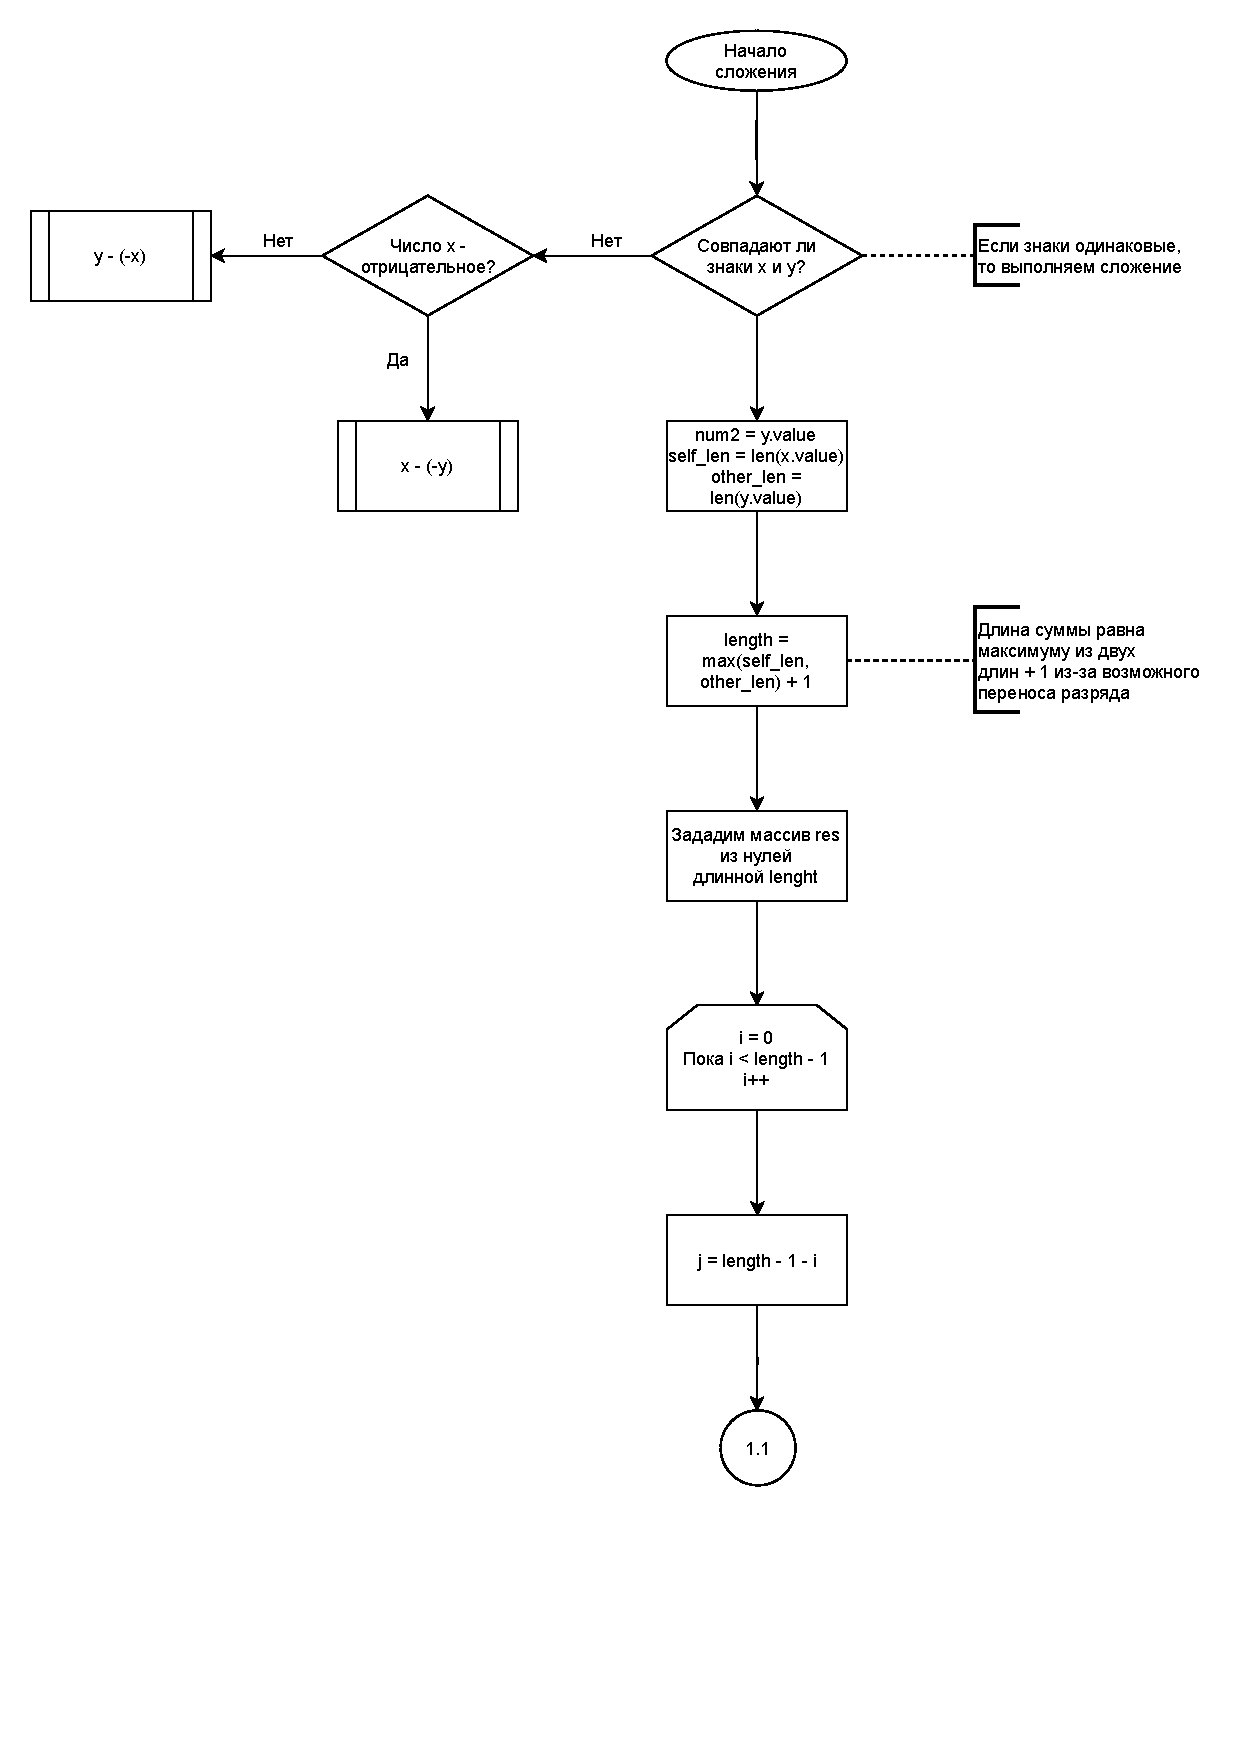
\includepdf[pages=-]{./Flowchart.pdf}
